\documentclass[USenglish]{ifimaster}

\usepackage[utf8]{inputenc}
\usepackage{ifimasterforside}
\usepackage{graphicx}
\usepackage[acronym]{glossaries}
\usepackage[backend=biber,sorting=none]{biblatex}

\usepackage{tabularx}
\usepackage{cleveref}

\makeglossaries

% Acronyms
\newacronym{afro}{AFRO}{Adaption Framework foR Web Services prOvision}
\newacronym{coap}{CoAP}{The Constrained Application Protocol}
\newacronym{cots}{COTS}{Commercial off-the-shelf}
\newacronym{dil}{DIL}{Disconnected, Intermittent and Limited}
\newacronym{ffi}{FFI}{Forsvarets forskningsinstitutt}
\newacronym{nec}{NEC}{Network Enabled Capability}
\newacronym{qos}{QoS}{Quality of Service}
\newacronym{rest}{REST}{Restful web services}
\newacronym{soa}{SOA}{Service-Oriented Architecture}
\newacronym{soap}{SOAP}{SOAP}
\newacronym{wsdl}{WSDL}{Web Services Description Language}
\newacronym{xml}{XML}{Extensible Markup Language}

\title{Improving the performance of Web Services in Disconnected, Intermittent
and Limited Environments}
\author{Joakim Johanson Lindquister}
\bibliography{references}

\begin{document}
\ififorside{}
\frontmatter{}

\chapter*{Abstract}
In this thesis I investigate different techniques to improve the performance of
Web services in typical tactical network environments.

\tableofcontents
\listoftables
\listoffigures

\pagebreak


\chapter{Introduction}
Military units may operate under conditions where the reliability of the network
connection is low. They can operate far from existing communication
infrastructure and rely only on wireless communication. Such networks are often
characterized by unreliable connections with low date rate and high error rates
making data communication difficult. In a military scenario it is necessary for
units at all operational levels to seamlessly exchange information across
different types of communication systems. To NATO, this concept is referred to
as \gls{nec}. In a feasibility study, NATO identified the \gls{soa} and Web
Services as key enablers\cite{nnec-study}.

Web services are well tested in civil environments where the network is stable
and the data rate is abundant. However, military networks may suffer from high
error rates and very low date rate, which can leave the Web services unusable.
This thesis investigate how these challenges can be overcome by applying
optimization techniques at different layers of the protocol stack.
%Ikke ta for gitt at sensor vet hva protocol stack er? Kanske forenkle eller
% utdype

\section{Background and Motivation}
NATO is a military alliance consisting of 28 member
countries\cite{nato-homepage-member-countries} and which primary goal is to
protect the freedom and security of its members through political and military
means. In joint military operations the relatively large number of member
countries can be a challenge when setting up machine-to machine information
exchange. Differences in communication systems and equipment can attribute to
make data exchange difficult. In order to address this issue, NATO has
chosen the \gls{soa} concept\cite{IST-090}.

\subsection{Service-Oriented Architecture}
\glsentryfull{soa} is an architectural pattern where application components
provide services to other components over a network. \gls{soa} is built on
concepts such as object-orientation and distributed computing and aims to get
a loose coupling between clients and services. In their reference model for
\gls{soa}\cite{oasis-soa-reference-model}, the Organization for the Advancement
of Structured Information Standards (OASIS) define \gls{soa} as: \paragraph{}
\textit{Service Oriented Architecture is a paradigm for organizing and utilizing
distributed capabilities that may be under the control of different ownership
domains. It provides a uniform means to offer, discover, interact with and use
capabilities to produce desired effects consistent with measurable preconditions
and expectations.} % SOA Trekant figur her

\paragraph{}
 In \gls{soa} business logic is divided into smaller chunks of logic, referred
 to as \textit{services}. A service can be business related, e.g a patient
 register service, or a infrastructure service used by other services and not by
 a user application.  Services are provided by \textit{service providers} and
 are consumed by \textit{service consumers}. The service provider is responsible
 for creating a service description, making the service available to others and
 implementing the service according to the service description. Services are
 made available to service consumers through a form of \textit{service
 discovery}. This can be a static configuration, or more dynamic with a central
 \textit{service registry}, where service providers publish service
 descriptions. Service consumers find the services they need by contacting the
 service registry. The communication between services occur through the exchange
 of standardized messages.

\begin{figure}[h]
\includegraphics[scale=0.6]{images/SOA.png}
\caption{The three roles in SOA(from \cite{IST-090})}
\end{figure}

Following the \gls{soa} principles dictates a very loose coupling between
services and the consumers of those. This allows software systems to be more
flexible, as new components can be integrated with minimal impact on the
existing system. Another aspect of loose coupling is with regard to time, which
enable services and its consumers to not be available at the same instance of
time. This enables asynchronous communication. Loose coupling with regards to
location allows the location of an service to be changed without needing to
reprogram, reconfigure, or restart the service consumers. This is possible
through the usage of service discovery, which is dynamically retrieval of the
new location of the service.

 Furthermore \gls{soa} enables service implementation neutrality. The
implementation of service is completely separated from the service description.
This allows re-implementation and alteration of a service without affecting the
service consumers. Thus this can attribute to keep development costs low and
avoiding proprietary solutions and vendor lock-in. Another benefit with
\gls{soa} is re-usability by dividing common business processes into services,
which may help cost reduction and avoids duplication. \gls{soa} is only a
pattern and the concepts can be realized by a range of technologies. The most
common used approach is the Web service familiy of standards, using the SOAP
messaging protocol. To achieve interoperability between systems from different
nations and vendors, NATO has chosen the Web Service technology in order to
realize the \gls{soa}  principles. This allows member nations to implement
their own technology as long as they adhere to the standards. The Web service
technology is discussed in detail in \cref{web-services}. Another approach to
\gls{soa} is \gls{rest}, which use HTTP over TCP. \gls{rest} has gained a lot
of traction in the civil industry and is discussed in section \cref{rest}.

\subsection{Military Networks}
% Trenger mer kjøtt her.
Web services can be used in strategic military networks as they have network
infrastructure with the same characteristics as civil networks.

\subsubsection{Tactical Networks}
Tactical networks are characterized by that the units are deployed to operate in
a battlefield, which means there is no existing communication infrastructure.
They use tactical communication equipment which includes technologies like VHF,
UHF, HF, tactical broadband and satellites\cite{IST-090}. % Mangler referanse på bruk av satelitter.
Examples of such units are mobile units like vehicles, foot soldiers and field
headquarters. The tactical network connects deployed headquarters with mobile
units. These types of networks are unpredictable and may have very low date
rate, possibly high delay, high error rates and frequent disconnections. They
are often called disadvantaged grids or \gls{dil} which is the term used in this
thesis. NATO studies have identified such networks to have the following
characteristics:
\\\\
\textit{
Disadvantaged grids are characterized by low bandwidth,variable throughput,
unreliable connectivity, and energy constraints imposed by the wireless
communications grid that link the nodes}\cite{nato-disadvantaged-grids}.
\paragraph{}
The characteristics of these networks and what challenges they impose are
discussed in detail in \cref{dil}.

\section{Problem Statement}
Most of the Web Service solutions used today are aimed for civilian use and do
not necessarily perform well in military environments. In contrast to civilian
networks where the date rate is abundant, mobile tactical networks may suffer
from high error rates and low date rate. Adapting Web service solutions meant
for civil networks directly for military purposes may not be possible.
Therefore, Web services needs to be adapted in order to handle network
challenges. However, it can be very expensive to alter existing Web service
technology and incorporate proprietary solutions. A NATO research task group has
previously identified the foundation on open standards to avoid tighter coupling
between service providers and consumers\cite{IST-090}. It is much better to use
\gls{cots} software. By placing the optimization in proxies, the
Web Services can remain unchanged.

The goal of this thesis is to investigate different optimization techniques that
can be applied in order to improve Web service performance in \gls{dil}
networks. In order for the clients and services to remain interoperable the
optimization techniques will be placed in proxies. The Web Services will
communicate as normal, while all network traffic is tunneled through a proxy.
The Web Service itself does not need to pay attention to the bad connectivity,
the proxy will choose the appropriate protocol and configuration.

\section{Premises}
The Web services and clients do not need to be changed.

\section{Scope and Limitations}
Snevre inn oppgaven.

Sikkerhet er ikke adressert i denne oppgaven(skal kanskje se på IPsec).

SOAP over HTTP klart det mest brukte, samt rest er utelukkende på HTTP. Derfor
støtter proxien kun HTTP ut og inn.

\section{Research Methodology}
Denning.


\section{Contribution}

The outcome of this thesis is a recommendation regarding which optimizations
techniques which can be used in DIL to enhance the performance of Web services.
Aswell as a prototype implementation of a DIL proxy.

\section{Outline}
Hvordan er resten av oppgaven strukturert.


%%%%% BACKGROUND %%%%
\chapter{Background}

%%%%%%%%%% DIL %%%%%%%%%%%%%%%
\section{\glsentrylong{dil}}
\label{dil}
The \gls{dil} concept refers to three characteristics of a network. As discussed
in the introduction, military tactical networks may suffer from these
constraints. These limitations are discussed in this section.

\begin{description}
\item[Disconnected]
Military units that participating in a tactical network are highly mobile
and may disconnect from a network either voluntarily or not. This causes
topology changes. Unplanned loss of connectivity can be due to various reasons,
such as loss of signal or equipment malfunction.  The disconnected term refers
to that nodes in the network may be disconnected for a long time, possibly for
multiple days.
\item[Intermittent]
Nodes in a \gls{dil} may loose connection temporarily before reconnecting. The
duration range from seconds to minutes.

\item[Limited] The Date rate, how many bits that are sent per second, is limited
in \gls{dil} networks. Various aspects that affects the date rate are discussed
in the next section.

\end{description}

\subsection{Network metrics}
\begin{description}

\item[Link throughput] The link throughput is influenced by how large distance
there is between the units communicating.

\item[Link reliability] How much of the arriving data that is correct. This is
called \textit{bit error rate} or \textit{packet error rate}. With high error
rates, more data to be transmitted again due to the data arriving being
incorrect. This contributes to longer transmission time. In a military setting,
an enemy may deliberate sabotage the network with jamming, causing higher error
rates.

\item[Link latency] The communication technology in use influences how fast data
transmission can be done. Long delay may cause that the application sending data
timing out.

\end{description}

\subsection{Other constraints}
Energy constraints imposed by the wireless communication grid. The battery
capacity and the transmission range of the communication equipment for mobile
units may be limited. Another issue is that in some cases military units are
required to enter radio silence in order to avoid being detected by the enemy.
During radio silence units may only receive data and not send any.


\section{Related Work}
Diskuterer eksisterende arbeid.

IST-090 ser på muligheten av å bruke SOA på taktisk nivå, med spesielt fokus på
disadvantged grids. Fokuserer på mulighet for Web services across disadvantaged
networks. Samt Data Distribution Service(DDS) på taktisk nivå.

In the report IST-090, a task group investigated solutions for making \gls{soa}
applicable at the tactical level. Three key issues that needs to be addressed in
order to apply Web Services in tactical networks was
identified\cite{IST-118}\cite{IST-090}:

\label{section:DIL-problems}

\subsubsection{End-to-end connections}

Web Services depend on a direct, end-to-end connection between the client and
the service. Attempting to establish and maintaining connections in DIL
environments can lead to increased communication overhead and possible complete
breakdown of communication. Most Web Services use TCP as the transport protcol,
which is a connection-oriented protocol designed for wired networks. In DIL
environments with high error rates and high latencies, the congestion control of
TCP will cause sub-optimal utilization of the network due to frequent connection
timeouts. Simmilar, HTTP, which is the application layer protocol most often
used together with TCP, struggeles in such enviroments. HTTP is a synchronous
protocol which means that the HTTP connection is kept open until a response is
received. Long response time cause timeouts. IST-090 points out the obivious
solution to replace HTTP and TCP with other, more suitable protocols.

The report mentions two approaches to replace HTTP/TCP. The clients and services
itself can be modified to support other protocols, or proxies which support
alternative protocols can be used. With employing a proxy solution, standards
complience can be retained.


\subsubsection{Network heterogeneity}

Another issuse is when heterogenous networks are interconnected. Different
performance in networks may lead to buildup of data in buffers, risking loss of
information. A proposed solution to this is to have store-and-forward support
which can support that messages are not dropped, but stored and forwarded when
possible.


\subsubsection{Web Service overhead}

Web services generate overhead as the Web Service technology is based on SOAP,
which use XML-based messages. It is a textual data format and produce much
larger messages than binary formats. Optimization approaches should seek to
reduce the network traffic generated by Web services by using techniques as
compression to reduce the size of messages. Another approach is to reduce the
number of messages being sent, which was looked into in IST-090\cite{IST-090}. In
their work they investigated three different ways to do this:

\begin{enumerate}
    \item Employing caching near the client in order to reuse older messages.
    \item Using publish/subscribe paradigm, which allows clients to subscribe to
    information instad of requesting it. This allows the same message to be sent
    to multiple clients.
    \item Employing content filtering, which filters out uneccessary data.
\end{enumerate}

\subsection{Proxies}


\subsubsection{DSProxy}

DSProxy is a proxy solution developed by \gls{ffi} which transports SOAP
messages over DIL networks. It reduces bandwidth needs by employing different
optimization techniques such as compression. It also provides delay tolerance
which allows \gls{cots} clients to function in DIL networks.


\subsubsection{AFRO}

\gls{afro} is an edge proxy which offers different levels of \gls{qos} to Web
Services through performance monitoring and application of the context-aware
service provision paradigm. It perform so called adaption actions, which
modifies the SOAP XML messages by changing their encoding to more efficient data
representation. It also cuts out information that are accepted to be removed by
the service requester. However, since the proxy modifies the data being sent,
the checksum of the data is also changed. In applications where we want to be
sure that no one has tempered with the data before arriving, checksums is often
used. Therefor this solution would not work for such applications.


\subsection{Configuration}
IST-90: Configure HTTP on the application server or ESP to prevent time-outs.
Anbefaler at hvis man trenger å gjøre propetiære optimaliseringer, så burde de
plasseres i proxier.


%%%%%%% WEB SERVICES
\section{Web services}
\label{web-services}
Web Services are client and server applications that communicate over a network
and can be used to implement a service-oriented architecture. All communication
is based on sending XML-based SOAP messages. There exists many definitions of
Web services where the core principles are the same, but the finer details may
vary. The World Wide Web Consortium has defined Web Services
as\cite{wrc-web-service}:
\paragraph{}
\textit{
    A Web service is a software system designed to support interoperable
    machine-to-machine interaction over a network. It has an interface described in
    a machine-processable format (specifically WSDL). Other systems interact with
    the Web service in a manner prescribed by its description using SOAP-messages,
    typically conveyed using HTTP with an XML serialization in conjunction with
    other Web-related standards.
}

\paragraph{}

This definition points out a set of standards that enables machine-to-machine
interactions. These standards are discussed in the following sections. The Web
Service technology, following the \gls{soa} principles, provides loouse coupling
and ease integration beteween systems. Figur her.


\subsection{XML}

\gls{xml} is a markup language and is considered as the base standard for Web
services. An XML document consist of data surrounded by tags and is designed to
be both machine and user readable. Tags describe the data they enclose. The tags
can be standarized, which allows exchange and understanding of data in a
standarized, machine-readable way.


\subsection{Service descriptions: WSDL}

\gls{wsdl} is an interface definition language that using XML describes
functionality offered by a Web Service. The interface describes available
functions, data types for message requests and responses and binding information
about the transport protocol, as well as address information for locating the
service. This enables a formal, machine-readable description of Web Service
which clients can invoke.


\subsection{SOAP}

\gls{soap} is an application level XML-based protocol specification for
information exchange in the implementation of Web services. It is transport
protocol agnostic and can be carried over various protocols. The far most
transport protocol used is HTTP over TCP, but other protocols such as UDP and
SMTP can be used as well. A SOAP message is an "envelope" consisting of an
optional header and a required body. The header can contain information not
directly related to the message such as routing information for the message and
security information. The body contains the data being sent, known as the
payload.

\subsection{\glsentrylong{rest}}
\label{rest}
However, there also exist other types of Web services which does not follow the
previously discussed standards. \glsentrylong{rest} let users manipulate data
using a set of stateless operations. \gls{rest} is easy to understand and has
gained a lot of traction in the civil industry in the latest years. \gls{rest}
uses exclusively HTTP over TCP. However, TCP does not necessarily perform
satisfactorily in \gls{dil} environments, which limits the usability in tactical
networks(trenger kilde?).


\section{Optimization techniques}
The Web service technology enable interoperability between systems, but also
increase the information overhead, requiring higher data rate demands. Employing
Web Services developed for use in civilian networks directly into a \gls{dil}
environment may not perform satisfactorily. To increase the performance we can
apply optimalization techniques. There are many approaches and optimalization
techniques which can be applied at different levels of the protocol stack. In
the coming sections the different optimization techniques are presented and a
overview is presented in \Cref{table:optimalization-overview}. Another issue
that needs to be addressed is, when we have identified optimization techniques,
where do we place them? In the application itself or in a proxy? This is
discussed in the next section.

\subsection{Where to place the optimalization?}
One approach is to modify the Web service application itself. However, this
would mean that every application that is used in a tactical network would
require modification. This would require a lot of resources and severely limit
the flexibility of using Web services. Another solution is, by using proxies, we
can place the optimization there without altering the Web Services themselves.
The only thing required to do is to setup the application to send and receive
data through the proxy. The proxy will take care of the optimization for
tactical networks. This seems like a more reasonable approach and is explored in
this thesis.


%%%%%%%% TABLE OPTIMALIZATION OVERVIEW %%%%%%%%%%%%%
\begin{table}[h]
\begin{tabularx}{\textwidth}{| X | X |}
\hline
  \textbf{Protocol Stack} & \textbf{optimization possibilities} \\ \hline
  The application & Optimize the application\\ \hline
  Web service messaging: SOAP & Optimize SOAP, e.g XML compression \\ \hline
  HTTP/TCP, UDP or other transport protocols & SOAP is transport agnostic. Other
  protocols can be used. \\ \hline
  IP & NATO NEC feasibility study states that all protocols should be over IP. \\
  \hline
  Lower layers & Not in the scope of this thesis. \\ \hline
\end{tabularx}
\caption{Optimization possibilities.} \label{table:optimalization-overview}
\end{table}


\subsection{Compressing the payload}
The first optimization techniques deals with the optimization of the encoding. By compressing the Web service payload, we can reduce the amount of data that need to be sent.
\begin{itemize}
\item GZIP
\item EFX(Efficient XML). XML spesefikt, får ikke brukt på REST når vi har andre
payloads..
\end{itemize}
Previous experiments shows EFX has the compression results with GZIP as the second best alternative\cite{johnsen-trude-compression-techniqes}.

\subsection{Reducing overhead of SOAP}
HTTP/TCP is the most used transport protocol for SOAP messages, but since SOAP is transport protocol agnostic different protocols can be used. Experiments show that this is possible.


%%%%%%%%%%%% Transport protokoller %%%%%%%%%%%%%%%%%%%
\begin{table}[h]
\begin{tabularx}{\textwidth}{| X | X |}
\hline
  \textbf{Transport Protocol} & \textbf{Summary} \\ \hline
  HTTP over TCP & Widely used. Breaks down in DIL environments.\\ \hline
  MQTT & Summary here\\ \hline
  Stream Control Transmission Protocol(SCTP) & Features multihoming. \\ \hline
  Advanced Message Queuing Protocol(AMPQ) & Application level protocol. Employs
  a broker architecture with store-and-forward capabilities. \\ \hline
  SOAP directly on TCP & Its possible \\ \hline
\end{tabularx}
\caption{Transport protocols}
\end{table}


\section{Transport Protocols}

\subsection{\glsentrylong{coap}}

\gls{coap} is a specialized web transfer protocol designed for use with
constrained nodes and constrained networks in the Internet of Things. It is
based on the REST model, where the server makes resources available  under a
URL. Clients access these resources using the HTTP-verbs GET, PUT, POST and
DELETE. Designed to use minimal resources, both on the device and on the
network.

\begin{itemize}
    \item Application level protocol.
    \item Can carry any data format.
    \item UDP on IP.
    \item Standardized in RFC 7252.
    \item Simple binary base header format
\end{itemize}


\subsection{AMQP}
AMQP is

\subsection{MQTT}
MQTT is

\subsection{SCTP}
SCTP is

\subsection{TCP}
TCP is

\subsection{UDP}
WSReliability?

For rest må det da bygges inn støtte i proxien.

Reliable UDP. Implmentasjon av UDP som er reliable. En gammel protokoll?


\section{Requirement Analysis}
A discussed in \cref{section:DIL-problems}, the dependency on end-to-end
connections needs to be removed. This can be done by adding proxies to the
network. Mobile units have to carry batteries with them and the capacity is
therefore limited. Advanced compression techniques may reduce the overhead, but
also requires more battery. This trade-off needs to be considered.
\\ \\ \\
\begin{table}[h]
\begin{tabular}{| l | l |}
\hline
  \textbf{Requirement} & \textbf{Priority} \\ \hline
  Receive and forward HTTP 1.X requests & 1\\ \hline
  Allow modifications on the payload & 1 \\ \hline
  Allow configuration of HTTP timeouts & 1 \\ \hline
  Keep HTTP-connection alive & 1 \\ \hline
  Support protocol X and y & 2 \\ \hline
\end{tabular}
\caption{Proxy requirements}
\end{table}

\section{Summary}



%%%% Design and implementation %%%%
\chapter{Design and Implementation}
\section{Overall Design}
\section{Proxy}
\subsection{Squid}
Squid is a fully-featured HTTP/1.0 proxy.
\begin{figure}[h]
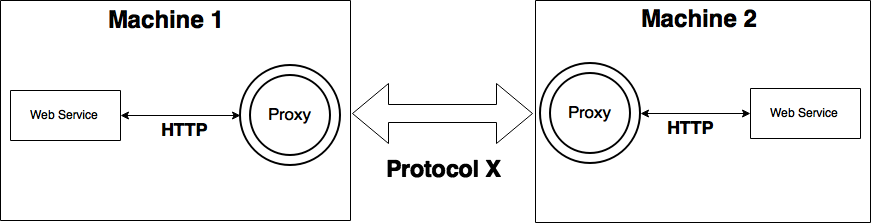
\includegraphics[scale=0.4]{images/architecture.png}
\caption{Architectural overview of proposed design}
\end{figure}

\subsection{Apache Camel}

\subsection{Tuning application server configuration}

\subsection{Alternative transport protocols}

\section{Summary}

\chapter{Testing and Evaluation}
\section{Evaluation Tools}

\chapter{Conclusion and Future Work}
\section{Conclusion}

\section{Future Work}

\pagebreak
\printbibliography{}
\printglossaries

\end{document}
